If a group of informed individuals are moving in the \emph{front line} of the group, these informed group will walk in a circular shape, making a quadratic bounding box surrounding them. 
The rest of the group will follow the informed group, so that if there are the same number of uninformed individuals as informed, they will together make up a bounding box with elongation of about 2, meaning that the side of the bounding box parallel to the direction is twice as long as the side perpendicular to the direction.
\newcommand{\figwidth}{0.21\textwidth}
\begin{figure}[H]
	\centering
	\begin{subfigure}[b]{\figwidth}
		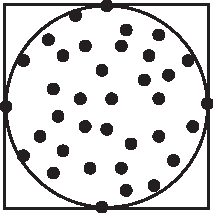
\includegraphics[width=\textwidth]{img/Circle.pdf}
		\caption{Actual distribution in box.\\\ }
		\label{fig:distr_true}
	\end{subfigure}
	~
	\begin{subfigure}[b]{\figwidth}
		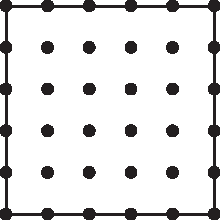
\includegraphics[width=\textwidth]{img/Square.pdf}
		\caption{Analytically approximated distribution}
		\label{fig:distr_approx}
	\end{subfigure}
	\caption{Approximation of particle distribution inside bounding box.}
	\label{fig:distr}
\end{figure}

\begin{figure}[H]
	\centering
	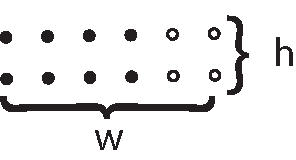
\includegraphics[width=0.24\textwidth]{img/heightwidth.pdf}
	\caption{Assumption of distribution when 4 out of 12 particles have information of destination. Circles indicates informed particles, solid dots indicates uninformed.}
	\label{fig:distr_direction}
\end{figure}
From the definition of Elongation, see \ref{sub:elongation}, we can put up a master equation for the elongation. With a distance between particles of length $\alpha$ we can define the parameters in Figure \ref{fig:distr_direction} as
\begin{align}
	h\cdot w &= N \\
	w &= (\sqrt{Np}-1)\alpha
\end{align}
The elongation can be calculated as 
\begin{equation}
	E = \frac{h}{w} = \frac{N}{(\alpha(\sqrt{Np}-1))^2}
\end{equation}

